\documentclass[11pt]{article}

\usepackage[margin=1in]{geometry}
\usepackage[T1]{fontenc}
\usepackage{lmodern}
\usepackage{microtype}
\usepackage{amsmath,amssymb,amsthm}
\usepackage{booktabs}
\usepackage[strings]{underscore}
\usepackage{hyperref}
\usepackage{xcolor}
\usepackage{listings}
\usepackage{tikz}
\usetikzlibrary{arrows.meta,positioning,fit,calc}

\hypersetup{
  colorlinks=true,
  linkcolor=blue!55!black,
  citecolor=blue!55!black,
  urlcolor=blue!55!black
}

\lstdefinelanguage{Lean}{
  keywords={def,theorem,structure,inductive,where,namespace,end,by,if,then,else,match,with,let,fun,import,abbrev},
  sensitive=true,
  morecomment=[l]{--},
  morecomment=[s]{/-}{-/},
  morestring=[b]"
}
\lstset{
  language=Lean,
  basicstyle=\ttfamily\small,
  keywordstyle=\color{blue!60!black},
  commentstyle=\color{gray!70!black},
  columns=fullflexible,
  keepspaces=true,
  frame=single,
  breaklines=true
}

\title{Machine-Checked Finite-Injury Priority Arguments:\\
Friedberg--Muchnik and Sacks Splitting in Lean 4}
\author{%
  Ara Aslyan\\
  Strike Technologies, New York\\
  \texttt{aaslyan@striketechnologies.com}
}
\date{}

\newcommand{\N}{\mathbb{N}}
% Renders as "c.e." at every use site, which always writes \ce followed by
% an explicit period (so that "\ce.\ set" spaces as a mid-sentence word).
\newcommand{\ce}{\ensuremath{\mathrm{c.e}}}
\newcommand{\leT}{\leq_T}

\begin{document}
\maketitle

\begin{abstract}
We describe a Lean 4 formalization of two finite-injury priority arguments
over a single, shared oracle-machine foundation: the Friedberg--Muchnik
theorem, which solves Post's problem by constructing two mutually
nonreducible computably enumerable sets, and the Sacks Splitting Theorem in
its splitting-with-non-reducibility form, which splits any non-computable
c.e.\ set into two c.e.\ halves computing neither.

The development is \emph{analytic} rather than synthetic: oracle
computation is not a black-box semantic relation but an explicit language
of oracle programs equipped with a step-indexed evaluator over finite
oracle information.  A halting bounded evaluation records both its output
and a strict upper bound on the oracle positions it queried, and the
central use theorem proves that such a computation is preserved under extra
fuel and under oracle agreement below the recorded use.  Restraint,
injury, initialization, attention, eventual stability and effective stage
construction are all represented directly, and computability of each stage
function is discharged against Mathlib's ordinary primitive- and
partial-recursive infrastructure.

The second theorem is a test of the first's foundation.  The whole
foundation transferred unchanged, and the recorded use---a design decision
taken for Friedberg--Muchnik---turned out to be what bounds the restraint
in Sacks, a theorem it was not designed for.  The priority layer did not
transfer at all: Friedberg--Muchnik's injury argument counts discrete
events, and a splitting requirement never acts, so a different induction is
required.  We report this as a negative result: ``finite injury'' names a
family of arguments rather than a single reusable lemma.  The two libraries
are siblings, importing a common foundation and not each other, and the
build enforces it.

Finally, we relate the local reducibility relation to Mathlib's own
\texttt{RecursiveIn} model by proving that every reduction there is
realized by a program of our language.  Since both conclusions are
negations of reducibility, this is the direction that rules out a
vacuously weak relation, and both theorems are restated over Mathlib's
notion.  The development builds with no \texttt{sorry}, and every headline
theorem depends only on \texttt{propext}, \texttt{Classical.choice} and
\texttt{Quot.sound}.

\end{abstract}

\section{Introduction}
\label{sec:intro}

\subsection{Two Kinds of Set}

Call a set of natural numbers \emph{decidable} if some algorithm, given a
number, answers yes or no and always terminates.  Call it \emph{computably
enumerable}, or \ce., if some algorithm lists its members --- possibly
forever, in no particular order, with no promise about when any given
member appears.  Every decidable set is \ce.; the converse fails, and the
standard witness is the halting problem, the set of programs that
eventually stop.  One can list the halting programs by running all of them
a step at a time and reporting each as it stops.  One cannot decide
membership, because a program that has not stopped yet may stop later, and
nothing in the enumeration says which.

The asymmetry is the subject.  A \ce.\ set carries \emph{positive}
information that accumulates: a number may join the set at some stage of
the enumeration, and once it joins it never leaves.  Negative information
never becomes final.  Every construction in this paper is a way of
exploiting that asymmetry, and every difficulty in formalizing one comes
from the same place.

To compare sets we relativize.  Give an algorithm a free subroutine --- an
\emph{oracle} --- that answers membership questions about a set $B$.  If
some such algorithm decides $A$, write $A \leT B$: $A$ is \emph{Turing
reducible} to $B$, meaning $A$ is no harder than $B$.  A halting oracle
computation asks its oracle only finitely many questions, all below some
bound called the \emph{use} of that computation.  This finiteness is the
one lever the whole theory turns on, and we return to it below.

Reducibility sorts sets into layers of difficulty.  At the bottom sit the
decidable sets, reducible to everything.  Near the top sits the halting
problem, to which every \ce.\ set reduces.

\subsection{Post's Problem}

In 1944 Post asked what lies between \cite{post1944}.  Is every \ce.\ set
either decidable or as hard as the halting problem, or is there something
strictly in the middle?

The question resisted for twelve years.  It was settled in 1956--57, by
Friedberg and by Muchnik independently \cite{friedberg1957,muchnik1956},
and settled in a strong form: there are two \ce.\ sets $A$ and $B$ with
$A \not\leT B$ and $B \not\leT A$.  Neither can decide the other, so
neither is decidable and neither is as hard as the halting problem.  The
middle is not merely occupied; it is occupied by incomparable things.

\begin{figure}[h]
\centering
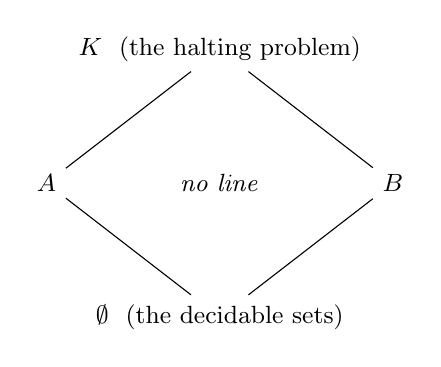
\begin{tikzpicture}[>=Stealth, every node/.style={font=\small}]
  \node (bot) at (0,0) {$\emptyset$ \ (the decidable sets)};
  \node (a) at (-2.2,1.7) {$A$};
  \node (b) at (2.2,1.7) {$B$};
  \node (top) at (0,3.4) {$K$ \ (the halting problem)};
  \draw (bot) -- (a);
  \draw (bot) -- (b);
  \draw (a) -- (top);
  \draw (b) -- (top);
  \node at (0,1.7) {\textit{no line}};
\end{tikzpicture}
\caption{The classical picture behind Post's problem: $A$ and $B$ sit
strictly between the decidable sets and the halting problem, and neither
reduces to the other.  The formalization reported here proves the two
missing edges --- $A\not\leT B$ and $B\not\leT A$ --- and proves that
neither set is decidable.  The halting problem itself does not appear in
the development, so the vertical placement in this diagram is classical
background rather than formalized content; see
Section~\ref{sec:scope}.}
\label{fig:degrees}
\end{figure}

A second classical result concerns how a \ce.\ set can be taken apart.
Sacks proved in 1963 that any \ce.\ set that is not decidable splits into
two disjoint \ce.\ pieces, neither of which can decide the whole
\cite{sacks1963}.  Nothing is thrown away --- the pieces reassemble to the
original --- and yet each piece has strictly less power than the set it
came from.  Both halves of the difficulty are genuinely present, and
neither half carries it alone.

\subsection{Why These Proofs Are Hard to Formalize}

Both results are proved by the same technique, introduced in the solution
of Post's problem and now called the \emph{priority method}.  It is worth
saying what the technique does before saying why it resists formalization.

To make $A \not\leT B$, one must defeat every candidate reduction.  Number
the oracle programs $\Phi_0, \Phi_1, \dots$ and impose one requirement per
program: $R_e$ says that $\Phi_e$ with oracle $B$ does not decide $A$.
Defeating a single $\Phi_e$ is easy in isolation.  Pick a number $x$ that
nothing else cares about --- a \emph{fresh witness} --- and keep it out of
$A$.  Watch $\Phi_e$ with oracle $B$ run on input $x$.  If it never
converges, it never decides $A$ and the requirement is met for free.  If it
converges and says ``$x \notin A$'', put $x$ into $A$.  Now the computation
is wrong, and the requirement is met by contradiction.

The difficulty is that the computation was run against $B$ \emph{as it
stood at that stage}, and $B$ is still being enumerated.  A later element
entering $B$ could change the computation and rescue it.  Here the finite
use is spent: the converging computation asked only finitely many questions
of $B$, so it suffices to \emph{restrain} $B$ below that use --- to promise
that no number smaller than the use will ever be enumerated into $B$.  The
computation is then frozen for good, and the diagonalization holds.

But restraints conflict.  A requirement that has promised to keep numbers
out of $B$ obstructs the requirements that want to put numbers in.  The
resolution is the priority ordering: requirements are ranked, and when a
higher-ranked one acts, every lower-ranked one is \emph{initialized} ---
its witness is discarded and its restraint cancelled, and it starts over
with a fresh witness chosen above the new restraint.  This is the
\emph{injury}.  The proof then argues that injury is finite: a requirement
is injured only by the finitely many stronger requirements above it, each
of which acts only finitely often, so eventually every requirement is left
alone forever and does its job.

This is a beautiful argument and an awkward one to make precise.  Its
content is carried by verbs in the future and past tense.  \emph{Choose a
witness nothing else cares about} --- nothing else meaning which
requirements, and cares in what sense, at which stage?  \emph{Wait until
the computation converges} --- waiting is not an operation; the
construction must at each stage make a decision from data it has, and
``converges'' is not such a datum, only ``converges within the resources
inspected so far''.  \emph{Restrain $B$ below the use} --- a promise about
all future stages, made at one stage, which some later stage must be shown
to keep.  \emph{Initialize everything weaker} --- an edit to unboundedly
many strategy records at once.  \emph{Eventually the stronger ones go
quiet} --- an induction along the priority order whose base case is that
the strongest requirement is never injured at all, and whose step needs a
measure of progress that no textbook states, because on paper it is
obvious.

In a proof assistant none of this can stay in the tense system.  Each
phrase has to become a piece of data or a theorem about it.  ``Fresh''
becomes a counter carried in the state and an invariant saying it dominates
everything mentioned so far.  ``Waiting'' becomes a decidable test on a
bounded execution, plus a separate theorem that a computation which really
does converge is eventually seen by that test.  ``Restraint'' becomes a
number in a record, plus a lemma that the enumeration respects it, plus the
preservation theorem that converts respect into a frozen computation.
``Initialize'' becomes an explicit rewriting of the strategy list.
``Eventually quiet'' becomes an induction along priority carrying an
explicit progress measure --- and finding that measure is real work, since
the informal proof supplies none.

That translation is the subject of this paper.  We report a Lean 4
formalization of both theorems --- Friedberg--Muchnik and Sacks splitting
in its splitting-with-non-reducibility form --- over one shared,
explicitly finitary model of oracle computation, and we report what the
translation cost and what it revealed.

\subsection{What This Paper Claims}
\label{sec:scope}

Our finding is not that the theorems are provable; they were proved
seventy years ago.  It is what happens when a second priority argument is
built on the first one's foundation.  The foundation transferred
completely, and one design decision made for the first theorem turned out
to be the load-bearing one for the second.  The priority layer transferred
not at all, and we argue that no generalization of it would have.  We
report that as a negative result about reuse: ``finite injury'' names a
family of arguments rather than a single reusable lemma.
Section~\ref{sec:formalization} is about both halves of that finding.

Two scope notes belong here rather than at the end.  First, what is
formalized is incomparability together with non-computability: for the two
constructed sets we prove $A \not\leT B$, $B \not\leT A$, and that neither
is decidable.  The classical step from there to ``strictly between
$\emptyset$ and the halting problem'' uses the fact that every \ce.\ set
reduces to the halting problem, and the halting problem, the jump, and
completeness do not appear in the development at all.  Figure~\ref{fig:degrees}
therefore shows more than we prove, and is labelled accordingly.  Second,
the full Sacks Splitting Theorem also makes the two halves \emph{low}; that
conclusion needs infinite-injury machinery and is deliberately out of
scope.  What we prove is the splitting-with-non-reducibility core.

\section{The Formalization and Its Key Decisions}
\label{sec:formalization}

The development is four Lean libraries.  \texttt{OracleComputability} fixes
a machine model of oracle computation and proves the facts any priority
argument over that model needs.  \texttt{FriedbergMuchnik} and
\texttt{SacksSplitting} are built on it, and neither imports the other;
Lake enforces this, so building either from a clean tree compiles no module
of the other.  \texttt{PriorityArguments} is a single root module joining
them.  The two headline theorems are:

\begin{lstlisting}
theorem friedberg_muchnik :
    exists A B : Set Nat,
      CE A /\ CE B /\ not (A <=T B) /\ not (B <=T A)

theorem sacks_splitting :
    forall A : Set Nat, CE A -> not (ComputableSet A) ->
      exists A0 A1, CE A0 /\ CE A1 /\ Disjoint A0 A1
        /\ A0 union A1 = A
        /\ not (A <=T A0) /\ not (A <=T A1)
\end{lstlisting}

The vocabulary --- \texttt{CE}, \texttt{ComputableSet}, and the relation
displayed as $\leT$ --- is defined in the shared library and imported by
both clients, not redefined, so the two theorems are stated in one
language.

\subsection{Deciding What Is Primary}

\paragraph{A finitary oracle model.}
The development does not start from a semantic type of oracle functionals.
Doing so would require an oracle-machine model, continuity or compactness
theorems, extraction of finite uses from semantic computations, and a
connection between functionals and executable indices --- all before the
first requirement could be stated.  Instead \emph{finite execution is
primary}.  The evaluator runs a concrete program for bounded fuel against a
partial oracle $\N \to \mathtt{Option}\ \mathtt{Bool}$, and returns one of
three outcomes: it halted, recording both its output and the use; it got
\emph{stuck}, having asked a question the finite oracle could not answer;
or it ran out of fuel.  Distinguishing the last two matters, because they
are repaired by different things --- more oracle information, or more
resources --- and a priority construction reacts to them differently.
Infinite computation is then defined as existence of a finite successful
run against a total oracle.

Recording the use inside the result, rather than recovering it afterwards
by a continuity argument, is the decision the rest of the development rests
on.  It makes the use principle a statement about data the construction can
inspect at a stage.  The principle itself, \texttt{run\_halt\_mono}, says
that a halting bounded run survives more fuel and any oracle that preserves
the answers it actually used.  The hypothesis is one-sided and deliberately
weak: positions at or above the recorded use are unconstrained, and so are
positions below the use where the original oracle had no information.  That
weakness is exactly what a restraint can deliver.

\paragraph{Finite sets, not Boolean prefixes.}
Evolving \ce.\ approximations are monotone finite sets, with Boolean lists
appearing only as bounded snapshots supplied to one computation:

\begin{lstlisting}
def StageMono (F : Nat -> Finset Nat) : Prop :=
  forall s, F s subset F (s + 1)

def limitSet (F : Nat -> Finset Nat) : Set Nat :=
  {n | exists s, n in F s}
\end{lstlisting}

The alternative --- representing an approximation as a prefix-monotone
Boolean string, where each bit is fixed once it appears --- is not merely
inconvenient, it proves the wrong theorem.  Fixing bits makes the limit
sets decidable, and the development proves that a decidable set reduces to
every oracle.  A prefix-monotone construction would therefore have handed
back precisely the reduction the theorem denies.  The two representations
coexist because they carry different information: a stage set may
accumulate new positive information at any later stage, while a snapshot
merely answers finitely many questions for one bounded run.

\paragraph{Where Mathlib enters, and where it does not.}
Ordinary, non-oracle computability is imported; oracle computability is
built locally.  Exactly three files import Mathlib's computability library:
one for the primitive-recursive closure theorems used to show the stage
functions computable, one embedding Mathlib's partial-recursive codes into
the query-free fragment of our language, and one relating our reducibility
to Mathlib's own oracle model.  The local oracle semantics --- the program
syntax, the evaluator, the use principle, the reducibility vocabulary, the
approximation layer --- mention Mathlib's codes nowhere, so changes to
Mathlib's internal coding decisions cannot reach them; the clients meet
Mathlib only where they must, in discharging computability of their stage
functions.  This
boundary lets the construction reason about explicit finite uses while
still reusing Mathlib's closure library \cite{carneiro2019,mathlibPartrec}.

\paragraph{Reducibility vocabulary.}
The central definition is that $A \leT B$ holds when some local oracle
program computes the characteristic function of $A$, on every input, from
the total characteristic function of $B$:

\begin{lstlisting}
def TuringReducible (A B : Set Nat) : Prop :=
  exists c : OracleCode,
    forall x : Nat,
      Computes c (charFun B) x (natOfBool (charFun A x))
\end{lstlisting}

Reflexivity, transitivity (by substituting one program for every query node
of another), and the fact that decidable sets reduce to every oracle are
all proved, so the relation is a preorder with the expected bottom
behaviour.  The program numbering is proved to be a bijection between $\N$
and the code type, which is what turns ``for every index $e$'' into ``for
every reduction'': the final diagonalization takes an arbitrary candidate
program, passes to its index, and lets the corresponding requirement kill
it.

\subsection{What Transferred to the Second Theorem, and What Did Not}
\label{sec:transfer}

The foundation was built for one theorem.  To test whether it was a
foundation rather than scaffolding, we formalized a second finite-injury
theorem against it and recorded, component by component and before writing
any of the second construction, what we expected to reuse.

\paragraph{The foundation transferred whole.}
Every component of the machine model, the use principle, the reducibility
vocabulary, the Mathlib bridge and the approximation layer was imported and
used unchanged.  Two items are worth naming.

The restraint lemma --- a computation seen halting against a stage snapshot
survives to the limit provided nothing below its recorded use is enumerated
later --- was already stated generically in the stage sequence rather than
in terms of the first construction's sets.  The preservation argument at
the heart of Sacks splitting therefore reuses it verbatim.  This was the
open question the reuse inventory was written to answer, and the answer is
clean.

More interestingly, the determinism lemma \texttt{run\_halt\_unique} carries
more weight in the second theorem than in the first.  In
Friedberg--Muchnik it says only that a computation has one output.  In
Sacks it is what makes \emph{the use of the limit computation at $y$} a
well-defined number, and that number is what bounds the restraint function.
Recording the use rather than only the output was a decision taken for the
first theorem, for reasons internal to it; it paid for a theorem it was not
designed for.  That is the strongest evidence we have that the foundation
generalizes.

\paragraph{The priority layer transferred not at all.}
The Friedberg--Muchnik injury argument counts \emph{events}.  A
requirement's record carries a rank in $\{0,1,2\}$ --- has it a witness,
has it acted --- receiving attention raises the rank strictly, and only
injury from above resets it.  So once the stronger requirements go quiet, a
requirement acts at most twice more.  This is the explicit progress measure
the informal proof does not supply, and it is small enough that the
induction along priority is arithmetic.

A splitting requirement generates no events.  It never acts: the elements
are not ours to choose, they arrive from the enumeration of the given set,
and the construction only decides which half each one joins.  Its restraint
moves continuously with the length of agreement between the reduction and
the set being split, so there is no discrete step to count and no rank to
raise.  The replacement is a three-part simultaneous induction along the
priority order: bounded restraints below $j$ give finite injury to $j$;
finite injury to $j$ gives satisfaction of $j$; satisfaction of $j$ bounds
$j$'s restraint.

The two arguments share a shape --- induction along the priority order, no
closed-form injury bound --- and no content.  The two files have no
declaration in common.  We looked for a common generalization worth stating
and did not find one, and we record that as a negative result about reuse
rather than as a defect of the first development's design: ``finite
injury'' names a family of arguments, not a single lemma one can prove once
and instantiate.

One further difference is forced by the mathematics rather than by taste.
The splitting restraint must be \emph{cumulative}, kept in the state as a
running maximum.  The raw stage restraint is not monotone --- the length of
agreement drops whenever a number below it enters the set --- and a
restraint that can drop protects nothing, since a computation frozen at one
stage could be destroyed later merely because its requirement had
temporarily stopped asking.  Friedberg--Muchnik needs no such device, its
restraint being written once, when a requirement acts.

\paragraph{Where the hypothesis is spent.}
Sacks splitting takes a hypothesis Friedberg--Muchnik does not have: the
set being split is not decidable.  The step that consumes it is the one
place where the second development required an argument with no analogue in
the first.  If a requirement is never injured after some stage and its
reduction nevertheless computes the characteristic function of $A$
everywhere, then $A$ is decidable: to decide $y \in A$, search for a stage
past the last injury whose length of agreement exceeds $y$, and report
whether $y$ is in the approximation at that stage.  Such a stage exists
because the reduction is total; the answer is correct because past the last
injury the agreeing computation is frozen by the restraint lemma, so it
\emph{is} the true value; and the search is effective because the whole
construction is primitive recursive.  Since $A$ is not decidable, no
requirement can be in that situation, so every requirement is satisfied.

Friedberg--Muchnik has no counterpart.  Its requirements are satisfiable
because their witnesses are fresh, which is a property of the construction;
a splitting requirement is satisfiable only because of a property of the
\emph{given} set.  We describe this as a step of the classical proof made
explicit rather than as new mathematics: it is the point at which a
textbook appeal to non-computability becomes a decision procedure that has
to be exhibited and shown effective.

\paragraph{What the second theorem cost.}
The shared foundation is roughly 2{,}870 lines; the Friedberg--Muchnik
client is roughly 2{,}000 and the Sacks client roughly 1{,}550.  The ratio
is the point: the expensive part --- model, evaluator, use principle,
Mathlib bridge, approximation layer --- was already present, and the second
theorem paid only for its own strategy.

Two components of the first development turned out to be artifacts of its
own design rather than necessities.  Its ten-field state invariant exists
to keep freely chosen witnesses fresh, distinct, and clear of
higher-priority restraints; a construction that does not choose its
elements needs none of it, and the two invariants that remain --- the
halves stay disjoint, and their union is the current stage of the given set
--- are one induction.  And its computability layer needs a shadow
implementation on plain tuples, because its state types are custom
structures with no \texttt{Primcodable} instance; defining the splitting
state as a tuple from the outset removes that layer, its simulation
theorem, and its list-surgery lemmas entirely.

The exercise also found two defects that only a second client could find.
Three generic helpers about primitive recursion had been declared
\texttt{private} inside the first development's computability file.
Nothing in them mentions either construction --- they are what any stage
function needs in order to be shown computable --- but \texttt{private}
made them invisible downstream.  Nothing needed generalizing; they needed
exporting.  Separately, the first development's root module imported a file
that did not exist, so a clean checkout did not build at all.  Its own
build never noticed, because the file was present locally.  Both are
invisible until someone tries to build on the code.

\subsection{Analytic, and Bridged Rather Than Asserted}
\label{sec:related}

Post's problem has been mechanized before, and the contrast is a design
decision rather than a survey obligation.  Zeng, Forster and Kirst
formalize a solution in Coq \cite{zeng2024post}, building on the synthetic
oracle computability of Forster, Kirst and M\"uck
\cite{forster2023oracle}.  Their setting is \emph{synthetic}: one works in
the Calculus of Inductive Constructions and takes every function
$\N\to\N$ to be computable by axiom, so there is no object-level machine
model and none of the details it brings.  That is a deliberate and
effective choice, and it answers the standard complaint that explicit
models of computation drown a computability proof in bookkeeping that stays
invisible on paper.  Two points of their work bear directly on ours: the
solution they formalize is Soare's low simple set, which their abstract
explicitly contrasts with ``the full Friedberg--Muchnik theorem
constructing two incomparable predicates''; and the same abstract records
that Bauer posed a synthetic proof of Friedberg--Muchnik as a challenge.

The present development is \emph{analytic}, and pays the cost the synthetic
approach avoids.  What is bought is that every informal appeal to
``preserve the computation below its use'' becomes an application of one
lemma about one evaluator, and that the resulting reducibility relation can
be compared with an external one by proof rather than by fiat.  Neither
approach dominates; they answer different questions about the same theorem.

That comparison is the last design decision.  Mathlib contains a model of
oracle computability \cite{mathlibTuringDegree}: an inductive relation
\texttt{RecursiveIn} on partial functions, Turing reducibility and
equivalence, and degrees as the quotient with a partial-order instance.  It
does not contain a use principle, oracle-relative step-indexed evaluation,
oracle-relative computable enumerability, or the jump, and it is not
connected to Mathlib's computably enumerable predicates, which live in a
separate file developed for the unrelativized theory.  The two libraries
are complementary: Mathlib has the degree \emph{structure} we do not build,
and we supply the finite-computation machinery it lacks.

So we prove the connection instead of assuming it.  A bridge file
establishes that every reduction in Mathlib's model is realized by a
program of our language, by induction over \texttt{RecursiveIn} with one
program per constructor.  This is the direction that matters: both of our
conclusions are \emph{negations} of reducibility, so the risk to guard
against is that our relation admits too few reductions and thereby makes
the negations cheap.  It does not, and both theorems are consequently
restated over Mathlib's relation.  The converse inclusion is not needed for
these results and is not proved.

Two priority claims, stated with the caution they deserve.  We are not
aware of another formalization of Post's problem in an analytic setting
with an explicit oracle machine model, nor of another in Lean; the
synthetic precedent above is the closest.  We are also not aware of any
formalization of the Sacks Splitting Theorem in any proof assistant.  Both
claims rest on a literature and repository search rather than an exhaustive
one, and neither is load-bearing for the technical content of this paper.

\subsection{The Shape of the Implementation}

The details of the machinery are tabulated in
Appendix~\ref{app:map}; what follows is the shape.

The program language is Kleene's schemata --- zero, successor, the two
projections, pairing, composition, primitive recursion and unbounded search
--- plus one oracle primitive, \texttt{query}, which asks whether its input
is in the oracle set.  A code with no \texttt{query} node is an ordinary
partial recursive program; the bridge embeds every Mathlib partial-recursive
code into that fragment and proves the embedding semantics-preserving, which
is the direction the construction consumes.  The evaluator's fuel discipline
deliberately copies
Mathlib's \texttt{evaln}, which is what lets the embedding be proved by a
single structural induction rather than by a simulation with fuel
translation.  The whole evaluator is proved primitive recursive, in the
form in which the construction consumes it: numbered codes in, encoded
results out.

The Friedberg--Muchnik construction keeps two enumeration lists, one record
per requirement holding a witness, an acted flag and a restraint, and a
freshness counter dominating everything mentioned so far.  At each stage
the least requirement requiring attention receives it: with no witness it
is given the counter's value; with an unacted witness whose diagonalizing
computation has appeared within the stage's resources, it acts ---
enumerating the witness, recording the computation's use as its restraint,
and resetting every weaker record.  A hypothesis-free case analysis proves
that every stage is exactly one of idle, appointment, or action, so no
execution path can escape the verification.  Ten invariants, proved
together by induction over those three transitions, carry the properties
the satisfaction proof cites by name, of which the load-bearing one says
that an acted requirement's diagonalizing computation still halts against
the current stage.

The splitting construction is smaller for a structural reason: it makes no
positive moves.  A stage takes the numbers the given set's own enumeration
has just produced and routes each to the half not being used as an oracle
by the strongest requirement that restrains it, defaulting to the first
half when nothing restrains it.  Two invariants suffice: the halves stay
disjoint, and their union is the current stage of the given set.

The computable-enumerability obligation is discharged the same way in both
developments and is the most expensive part of each.  The stage function is
shown primitive recursive using Mathlib's closure library, an unbounded
search over stages turns it into a partial recursive semi-decider, and the
bridge converts that into the project's \texttt{CE}.  For
Friedberg--Muchnik this requires the shadow tuple implementation and a
simulation theorem tying it to the real machine, and it dominates the build:
one file accounts for roughly seven eighths of the project's compile time.
The instructive failure along the way was assembling that derivation as a
single large combinator term, which made failed unifications fall back into
the pairing encodings and left the elaborator symbolically evaluating
arithmetic for tens of millions of heartbeats.  Confining each
tuple-sized comparison to its own lemma fixed it.

\section{Conclusion}
\label{sec:conclusion}

Two classical finite-injury priority arguments are formalized in Lean 4
over one explicitly finitary model of oracle computation.  The informal
temporal reasoning of the textbook proofs --- choose a fresh witness, wait
for convergence, restrain below the use, initialize what is weaker, argue
that the stronger requirements eventually go quiet --- becomes finite
executable stages, explicit state components, recorded uses, preserved
invariants, a bounded progress measure, and an induction along priority.
The constructions are not merely type-checked but executable: the stage
machines run, and produce the witnesses, restraints and enumerations the
proofs reason about.

The methodological lesson is about representation.  Priority arguments are
not beyond current provers, but they require representations that expose
finite information at exactly the points where the informal proof appeals
to it.  Recording the use inside the evaluator's result, rather than
recovering it after the fact, is what makes restraint a manipulable object;
keeping approximations as monotone finite sets rather than prefix-fixed
Boolean strings is what keeps the limit sets from being decidable and the
theorem from being false.

The second lesson is the one we did not expect, and it is negative.  A
foundation built for one priority argument served a second one completely
--- including a lemma whose importance in the second theorem exceeds its
importance in the first --- while the priority layer itself transferred not
at all, and no generalization of it appears to be worth stating.  ``Finite
injury'' names a family of arguments related by shape, not a lemma one
proves once.  A useful reusable priority framework, if there is one, will
have to abstract requirements, strategies, priority order, initialization
and progress measures at a level neither of these two developments
currently occupies; we regard that as open rather than as routine
engineering.

The natural next target is infinite injury.  It is what the omitted
conclusion of the Sacks Splitting Theorem needs --- lowness of the two
halves --- and it is the first place where the finite progress measure that
made the first theorem tractable is unavailable in principle rather than by
accident of design.  The other loose ends are smaller.  Transitivity of the
local reducibility relation, listed as future work in an earlier draft of
this development, is now proved by query substitution, so the relation is a
preorder; what remains is that the bridge to Mathlib's oracle model is
proved in one direction only, which suffices for the negative results here
but not for a general transfer, and that no degree structure --- the
quotient, the jump, completeness --- is formalized, so the classical
reading of these theorems as statements about degrees remains external to
the artifact.


\bibliographystyle{plain}
\bibliography{references}

\appendix
\section{Textbook-to-Lean Map}

\begin{table}[h]
\centering
\small
\begin{tabular}{llll}
\toprule
Textbook concept & Lean representation & Main declaration & File \\
\midrule
Oracle program & program syntax & \texttt{OracleCode} & \texttt{Foundation/OracleCode.lean} \\
Finite computation & bounded evaluator & \texttt{run} & \texttt{Foundation/FiniteEval.lean} \\
Output/use & halting data & \texttt{HaltData} & \texttt{Foundation/FiniteEval.lean} \\
Use preservation & agreement below use & \texttt{run\_halt\_mono} & \texttt{Foundation/Use.lean} \\
Infinite computation & existential finite run & \texttt{Computes} & \texttt{Foundation/InfiniteEval.lean} \\
Program enumeration & code numbering & \texttt{ofNatCode\_encodeCode} & \texttt{Foundation/Numbering.lean} \\
c.e. approximation & monotone stages & \texttt{StageMono} & \texttt{Approximation.lean} \\
Limit set & union of stages & \texttt{limitSet} & \texttt{Approximation.lean} \\
Requirement state & strategy record & \texttt{ReqState} & \texttt{Construction.lean} \\
Witness & strategy field & \texttt{witness} & \texttt{Construction.lean} \\
Restraint & strategy field & \texttt{restraint} & \texttt{Construction.lean} \\
Attention & stage predicate & \texttt{requiresAttention} & \texttt{Construction.lean} \\
Priority action & deterministic step & \texttt{stepAt}, \texttt{stepState} & \texttt{Construction.lean} \\
No upward injury & record preservation & \texttt{reqs\_getElem?\_succ\_of\_lt} & \texttt{StageDynamics.lean} \\
Invariant package & construction invariant & \texttt{ConsInv}, \texttt{consInv\_stage} & \texttt{Invariants.lean} \\
Finite injury & eventual quietness & \texttt{quiet\_above} & \texttt{FiniteInjury.lean} \\
Stabilization & final record & \texttt{exists\_stable} & \texttt{FiniteInjury.lean} \\
Diagonalization & requirement satisfaction & \texttt{R\_satisfied}, \texttt{S\_satisfied} & \texttt{Requirements.lean} \\
c.e. limit set & semidecision & \texttt{ce\_Aset}, \texttt{ce\_Bset} & \texttt{CE.lean} \\
Final theorem & assembly & \texttt{friedberg\_muchnik} & \texttt{Main.lean} \\
\bottomrule
\end{tabular}
\caption{Mapping between textbook proof concepts and Lean declarations.}
\end{table}


\section{Verified Artifact Facts}
\label{app:facts}

Every figure below was measured against the repository, on a clean build,
rather than asserted.  Measurements are from an Apple M5 (10 cores, 32~GB)
with Mathlib's compiled artifacts supplied by \texttt{lake exe cache get}.

\begin{table}[h]
\centering
\small
\begin{tabular}{ll}
\toprule
Item & Value \\
\midrule
Lean toolchain & \texttt{leanprover/lean4:v4.26.0} \\
Mathlib version & \texttt{v4.26.0} \\
Mathlib revision & \texttt{2df2f0150c275ad53cb3c90f7c98ec15a56a1a67} \\
Lake libraries & 4 \\
Lean files & 30 \\
Lines of Lean & 6{,}499 \\
Lines excluding comments and blanks & 4{,}471 \\
Hand-written \texttt{theorem} declarations & 274 \\
Hand-written \texttt{def}/\texttt{abbrev} declarations & 90 \\
\texttt{lake build} & succeeds, 829 jobs \\
Clean build, Mathlib cached & 2\,min 2\,s \\
Slowest module (\texttt{FriedbergMuchnik/CE.lean}) & 106\,s \\
Declarations checked with \texttt{\#print axioms} & 37 \\
Axiom footprint, all 37 & \texttt{propext}, \texttt{Classical.choice}, \texttt{Quot.sound} \\
Axioms declared by the development & 0 \\
\texttt{sorry} / \texttt{admit} & 0 \\
\texttt{native\_decide} / \texttt{unsafe} / \texttt{partial def} & 0 \\
\texttt{noncomputable} declarations & 2 \\
Declarations with raised \texttt{maxHeartbeats} & 11 \\
Repository license & none \\
CI workflow & none \\
\bottomrule
\end{tabular}
\caption{Artifact facts, measured at the revision described in
Appendix~\ref{app:artifact}.}
\end{table}

\begin{table}[h]
\centering
\small
\begin{tabular}{lrrr}
\toprule
Library & Files & Lines & Code lines \\
\midrule
\texttt{OracleComputability} & 14 & 2{,}866 & 2{,}000 \\
\texttt{FriedbergMuchnik} & 8 & 2{,}002 & 1{,}494 \\
\texttt{SacksSplitting} & 7 & 1{,}548 & 948 \\
\texttt{PriorityArguments} & 1 & 83 & 29 \\
\bottomrule
\end{tabular}
\caption{Size by library.  ``Code lines'' excludes comments and blanks.}
\end{table}

The two \texttt{noncomputable} declarations are the classical
characteristic function \texttt{charFun}, which appears only in the
statements of the reducibility vocabulary, and \texttt{limUse}, which
appears only in the verification of the second theorem.  Neither occurs in
a construction.  The raised heartbeat budgets are elaboration limits in the
two computable-enumerability files and cannot affect the axiom footprint,
which is the ground truth that no logical shortcut was taken.

\paragraph{The constructions run.}
Both stage machines are executable Lean functions, and evaluating them is a
stronger check than the absence of \texttt{sorry}: it shows the definitions
are not vacuously satisfiable stubs.  Evaluating the Friedberg--Muchnik
machine --- the one the priority proof reasons about, not the shadow
implementation used for the computability proof --- at stage 20 gives
enumerations $\{12,8,6,4,0\}$ and $\{13,10,1\}$ for the two sets, a
freshness counter of $14$, and strategy records in which requirements 8 and
10 hold restraints 9 and 11 respectively.  Evaluating the splitting machine
on the code that halts everywhere routes the first eight elements into a
single half, all restraints remaining zero, since a reduction that always
answers zero never agrees with a set that is accumulating members.

\section{Artifact Reproduction}

The repository is available at:

\begin{verbatim}
https://github.com/aaslyan/friedberg-muchnik-lean
\end{verbatim}

A fresh build should use:

\begin{verbatim}
git clone https://github.com/aaslyan/friedberg-muchnik-lean
cd friedberg-muchnik-lean
lake exe cache get
lake build
\end{verbatim}

To check the final theorem and axiom footprint:

\begin{verbatim}
cat >/tmp/check_fm.lean <<'EOF'
import FriedbergMuchnik.Main

#check FriedbergMuchnik.friedberg_muchnik
#print axioms FriedbergMuchnik.friedberg_muchnik
EOF

lake env lean /tmp/check_fm.lean
\end{verbatim}

At drafting time this reported:

\begin{verbatim}
FriedbergMuchnik.friedberg_muchnik :
  exists A B,
    FriedbergMuchnik.CE A /\
      FriedbergMuchnik.CE B /\
        not FriedbergMuchnik.TuringReducible A B /\
        not FriedbergMuchnik.TuringReducible B A
'FriedbergMuchnik.friedberg_muchnik' depends on axioms:
  [propext, Classical.choice, Quot.sound]
\end{verbatim}

To search for common proof escape hatches:

\begin{verbatim}
rg -n "sorry|admit|axiom|unsafe|opaque|extern|implemented_by|native_decide" \
  FriedbergMuchnik FriedbergMuchnik.lean lakefile.lean README.md STATUS.md
\end{verbatim}

At drafting time this command found only documentation mentions of
\texttt{sorry}/\texttt{axiom}, not source declarations.



\end{document}
